\documentclass[12pt,a4paper]{article}

% --- Layout (conforme SBC: A4, 1 coluna, margens) ---
\usepackage[a4paper,top=3.5cm,bottom=2.5cm,left=3.0cm,right=3.0cm]{geometry}
\usepackage{times}
\usepackage[T1]{fontenc}
\usepackage[utf8]{inputenc}
\usepackage[brazil]{babel}

% --- Figuras/Tabelas ---
\usepackage{graphicx}
\usepackage{booktabs}
\usepackage{url}
\usepackage{microtype}
\usepackage{float}
\usepackage{xcolor}
\usepackage{helvet}
\usepackage[font={bf,small},labelfont=bf]{caption} % aproxima estilo SBC (Helvetica 10 bold)

\title{\textbf{Descrição e Análise Inicial da Base \texttt{bd2\_sistema\_e\_saude}}}
\author{\textbf{Aluno(a) UTFPR}\\
Banco de Dados -- Tarefa 3\\
\texttt{seu.email@exemplo.com}}
\date{}

\begin{document}
\maketitle

\begin{abstract}
Este relatório apresenta a tabela \texttt{public.bd2\_sistema\_e\_saude} (PostgreSQL), descrevendo seus atributos, volume de dados e problemas encontrados na inserção/modelagem. Em seguida, propõe perguntas básicas e avançadas e indica a melhor forma (tabela/gráfico) de responder cada uma, utilizando visualizações geradas automaticamente em \texttt{output/}.
\end{abstract}

\noindent\textbf{Resumo.}
Este relatório apresenta a tabela \texttt{public.bd2\_sistema\_e\_saude} (PostgreSQL), descrevendo seus atributos, volume de dados e problemas encontrados na inserção/modelagem. Em seguida, propõe perguntas básicas e avançadas e indica a melhor forma (tabela/gráfico) de responder cada uma, utilizando visualizações geradas automaticamente em \texttt{output/}.

\section{Descrição da tabela e dos atributos}
\subsection{Visão geral}
A base analisada está armazenada no banco \texttt{postgiscwb}, na tabela \texttt{public.bd2\_sistema\_e\_saude}. O conjunto contém \textbf{2.256.598} tuplas (contagem no banco) com atributos clínicos e administrativos (ex.: data do atendimento, unidade, localização e CID).

\subsection{Atributos (resumo)}
A tabela possui dezenas de colunas. A Tabela~\ref{tab:atributos} lista os atributos mais relevantes para a análise inicial e os respectivos tipos.

\begin{table}[H]
\centering
\caption{Atributos principais e tipos (resumo).}
\label{tab:atributos}
\begin{tabular}{ll}
\toprule
\textbf{Atributo} & \textbf{Tipo (PostgreSQL)} \\
\midrule
\texttt{data\_do\_atendimento} & \texttt{timestamp} \\
\texttt{data\_de\_nascimento} & \texttt{timestamp} \\
\texttt{sexo} & \texttt{varchar(1)} \\
\texttt{tipo\_unidade}, \texttt{codigo\_unidade} & \texttt{varchar(50)}, \texttt{varchar(150)} \\
\texttt{bairro}, \texttt{municipio} & \texttt{varchar(72)}, \texttt{varchar(50)} \\
\texttt{codigo\_cid}, \texttt{descricao\_cid} & \texttt{varchar(4)}, \texttt{varchar(150)} \\
\texttt{codigo\_procedimento} & \texttt{varchar(12)} \\
\texttt{encaminhamento\_especialista} & \texttt{varchar(3)} \\
\midrule
\textit{Observação} & Demais colunas: procedimento/CBO, \\
 & variáveis socioambientais e flags. \\
\bottomrule
\end{tabular}
\end{table}

\subsection{Exemplo de tupla}
A Tabela~\ref{tab:tupla} apresenta um exemplo real (com \texttt{cod\_usuario} mascarado) para ilustrar o formato dos dados.

\begin{table}[H]
\centering
\caption{Exemplo de tupla extraída da base (campos selecionados).}
\label{tab:tupla}
\begin{tabular}{ll}
\toprule
\textbf{Campo} & \textbf{Valor} \\
\midrule
\texttt{data\_do\_atendimento} & 2024-10-04 10:33:39 \\
\texttt{data\_de\_nascimento} & 1994-06-27 03:00:00 \\
\texttt{sexo} & M \\
\texttt{tipo\_unidade} & BASICO \\
\texttt{codigo\_unidade} & 5406617 \\
\texttt{codigo\_cid} & Z760 \\
\texttt{bairro} & CAMPO COMPRIDO \\
\texttt{municipio} & CURITIBA \\
\texttt{cod\_usuario} & 12*** \\
\bottomrule
\end{tabular}
\end{table}

\section{Problemas encontrados na inserção/modelagem}
O principal desafio foi definir uma \textbf{chave primária} (PK). Nenhum atributo isolado se mostrou suficiente para unicidade. Foi necessário testar chaves compostas até obter um conjunto que evitasse duplicidades. A PK definida foi:
\[
(\texttt{data\_do\_atendimento},\ \texttt{codigo\_unidade},\ \texttt{codigo\_cid},\ \texttt{cod\_usuario})
\]
Além disso, ao iniciar o uso de migrations com TypeORM, diferenças entre \texttt{varchar} com/sem \texttt{length} e ausência de índices na Entity faziam o gerador de migrations propor alterações agressivas. A Entity foi ajustada para refletir 100\% do schema (incluindo \texttt{length} e \texttt{@Index}).

\section{Descrição dos dados e perguntas de análise}
Nesta seção, são propostas \textbf{5 perguntas básicas} e \textbf{2 avançadas}, indicando a melhor forma de resposta (tabela/gráfico). Figuras citadas foram geradas pelos scripts do projeto e salvas em \texttt{output/}.

\subsection{Perguntas básicas (5)}
\begin{itemize}
  \item \textbf{(B1) Como o volume de atendimentos varia ao longo do tempo?} \textit{(gráfico de linha mensal)}.
  \item \textbf{(B2) Qual é o perfil etário dos atendimentos?} \textit{(histograma por faixas)}.
  \item \textbf{(B3) Quais bairros concentram mais atendimentos?} \textit{(barras horizontais Top N)}.
  \item \textbf{(B4) Quais municípios concentram mais atendimentos?} \textit{(barras horizontais Top N)}.
  \item \textbf{(B5) Como o volume se distribui por mês e tipo de unidade?} \textit{(barras empilhadas)}.
\end{itemize}

\begin{figure}[H]
\centering
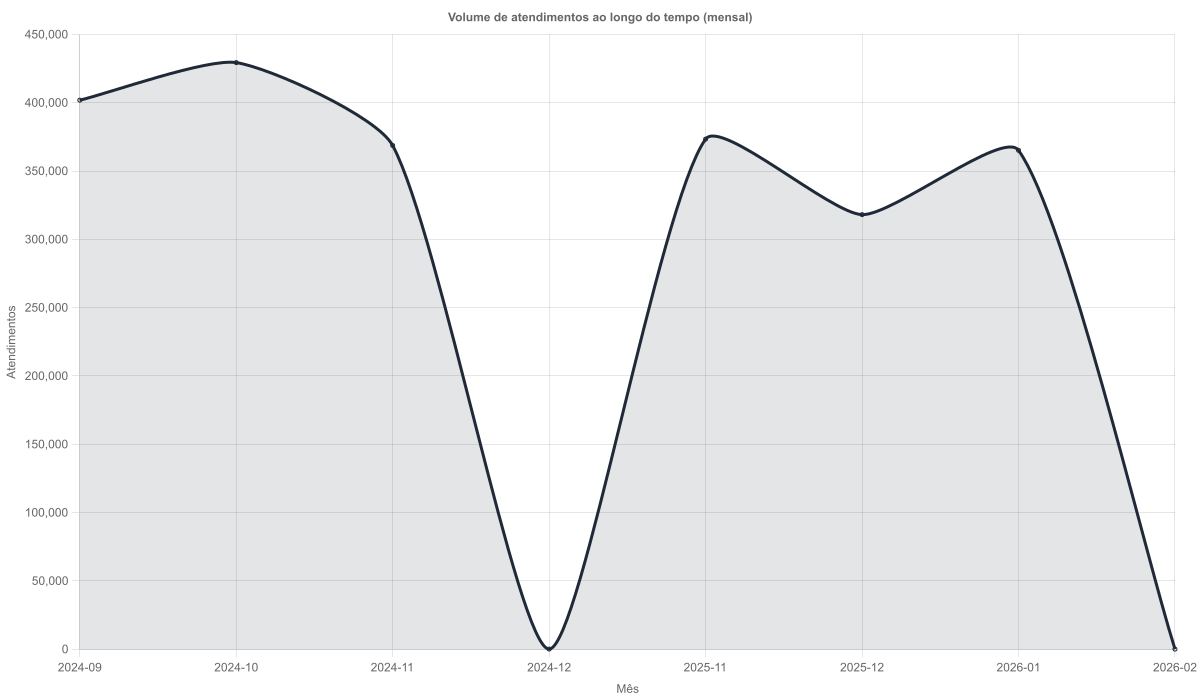
\includegraphics[width=0.48\textwidth]{output/volume-atendimentos-mensal.png}\hfill
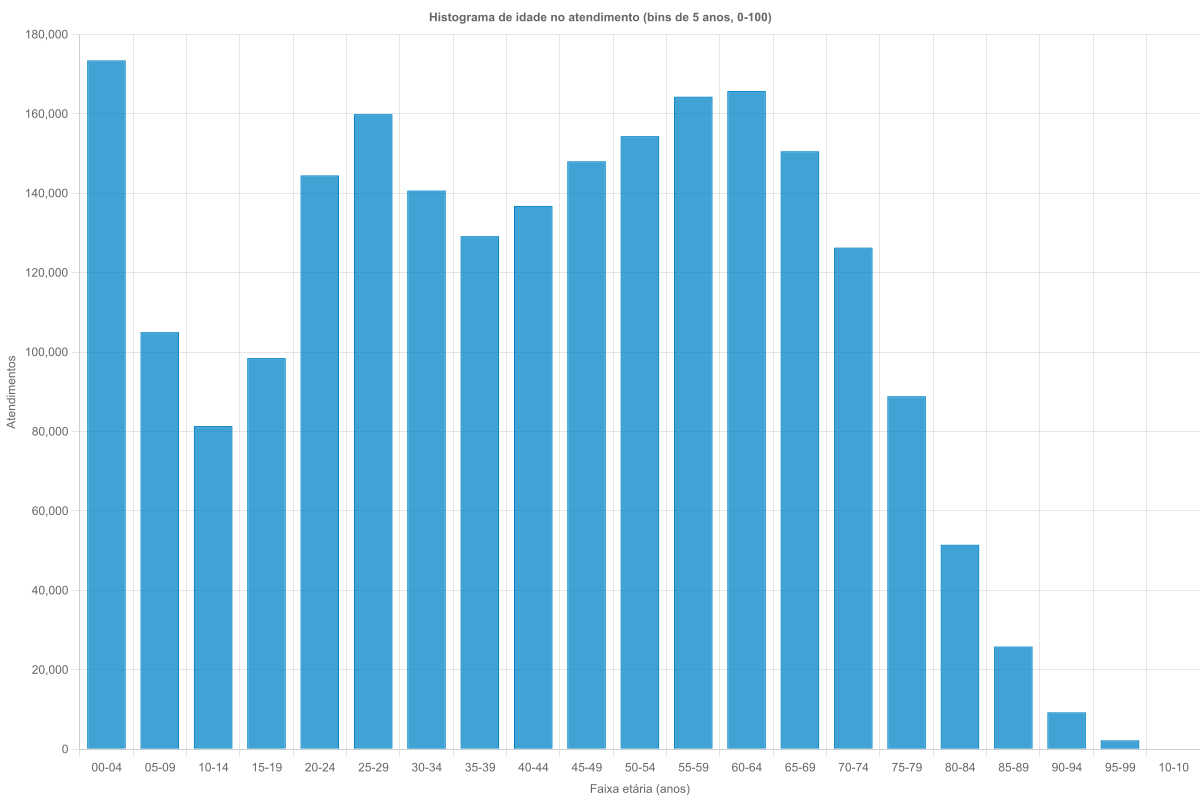
\includegraphics[width=0.48\textwidth]{output/idade-histograma.png}
\caption{(Esq.) Volume mensal de atendimentos (B1). (Dir.) Histograma de idade no atendimento (B2).}
\label{fig:b1b2}
\end{figure}

\begin{figure}[H]
\centering
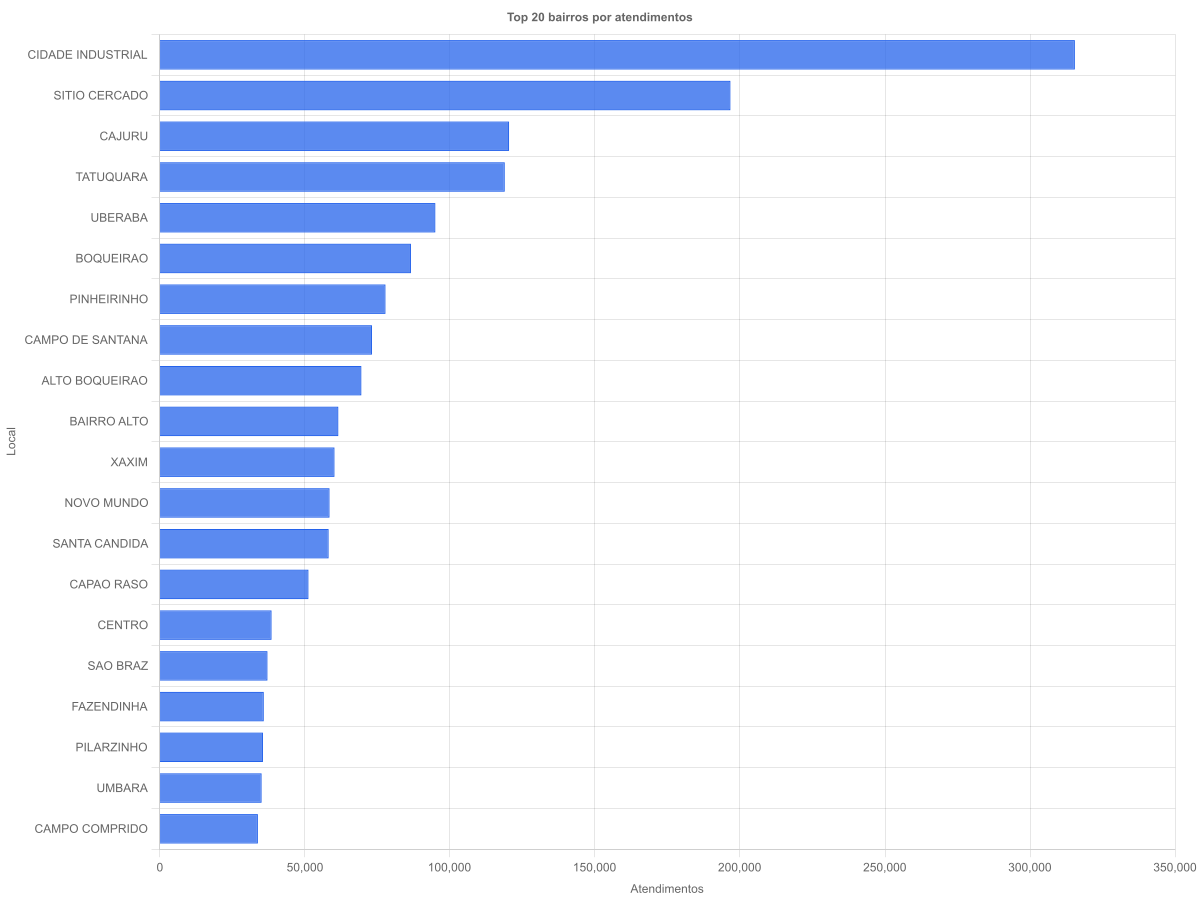
\includegraphics[width=0.48\textwidth]{output/top-bairros.png}\hfill
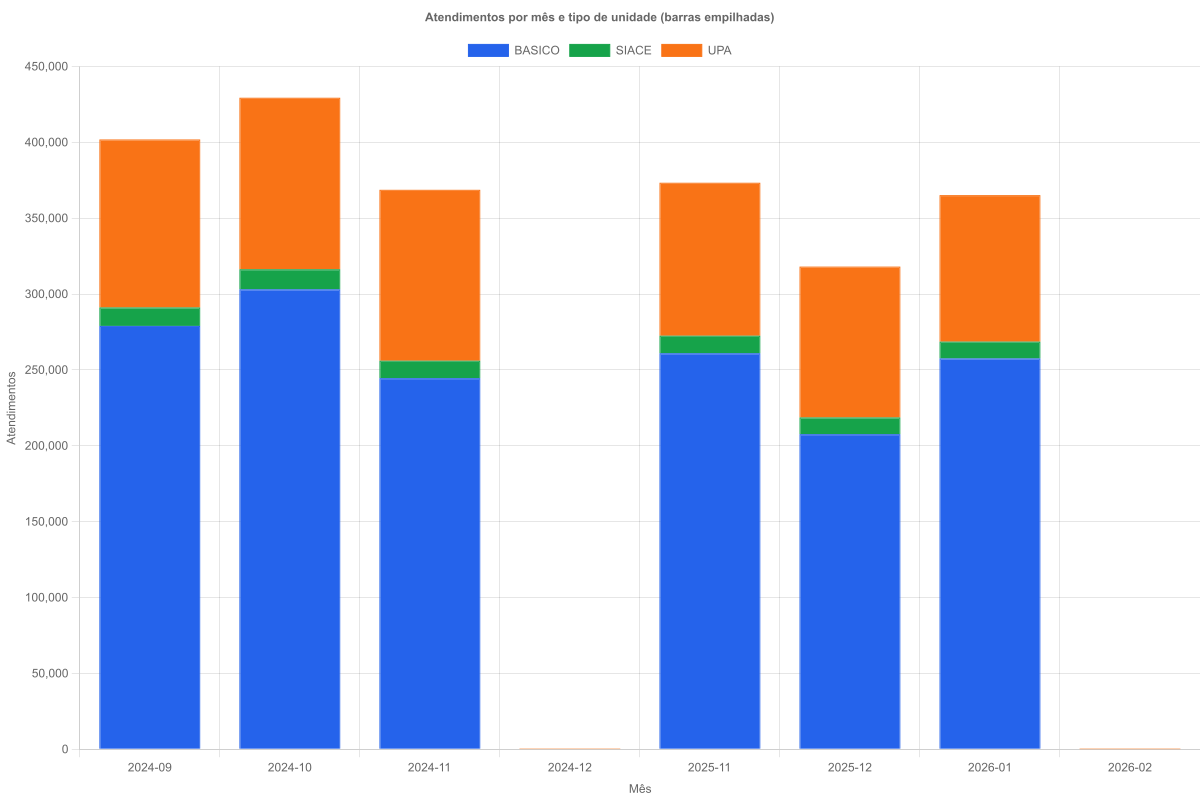
\includegraphics[width=0.48\textwidth]{output/tipo-unidade-por-mes.png}
\caption{(Esq.) Top bairros por atendimentos (B3). (Dir.) Atendimentos por mês e tipo de unidade (B5).}
\label{fig:b3b5}
\end{figure}

\subsection{Perguntas avançadas (2) com fatores ambientais}
\begin{itemize}
  \item \textbf{(A1) Chuva/precipitação altera o volume e o perfil dos atendimentos?}
  \textit{Melhor forma}: tabela diária (atendimentos + precipitação) e gráfico de dispersão/boxplot por faixas de chuva, com análise de defasagens (lags) de 1--7 dias.
  \item \textbf{(A2) Ruído urbano se associa à maior frequência de certos CIDs (ex.: cefaleia) ou à maior demanda por tipo de unidade?}
  \textit{Melhor forma}: cruzamento por bairro/mês (ruído + taxa de CID), com gráfico de dispersão e/ou mapa de calor (bairro $\times$ mês). Recomenda-se normalizar por população quando disponível.
\end{itemize}

\section{Reprodutibilidade}
As figuras básicas foram geradas com os comandos:
\texttt{npm run chart:volume}, \texttt{npm run chart:idade}, \texttt{npm run chart:top-locais} e \texttt{npm run chart:tipo-unidade}.

\noindent\textbf{Observação sobre PDF.} No ambiente atual não há \texttt{pdflatex} disponível. O arquivo \texttt{relatorio\_sbc.tex} foi produzido seguindo o template SBC (A4, 1 coluna, margens e estilo) e pode ser compilado em um ambiente \LaTeX\ (ex.: Overleaf ou TeX Live) para gerar o PDF final.

\end{document}

